\documentclass[10pt]{beamer}
\usepackage[latin1]{inputenc}
\usepackage[T1]{fontenc}
\usetheme{metropolis}
\usepackage{appendixnumberbeamer}

\usepackage{booktabs}
\usepackage[scale=2]{ccicons}

\usepackage{algorithm2e}
\usepackage{pgfplots}
\usepgfplotslibrary{dateplot}
\usepackage{subcaption}
\usepackage{pbox}
\usepackage{xspace}
\definecolor{mygreen}{rgb}{0,0.6,0}
\definecolor{mygray}{rgb}{0.5,0.5,0.5}
\definecolor{mymauve}{rgb}{0.58,0,0.82}
\usepackage{listings}
\lstset{ %
  backgroundcolor=\color{white},   % choose the background color; you must add \usepackage{color} or \usepackage{xcolor}; should come as last argument
  basicstyle=\footnotesize,        % the size of the fonts that are used for the code
  breakatwhitespace=false,         % sets if automatic breaks should only happen at whitespace
  breaklines=true,                 % sets automatic line breaking
  captionpos=b,                    % sets the caption-position to bottom
  commentstyle=\color{mygreen},    % comment style
  deletekeywords={...},            % if you want to delete keywords from the given language
  escapeinside={\%*}{*)},          % if you want to add LaTeX within your code
  extendedchars=true,              % lets you use non-ASCII characters; for 8-bits encodings only, does not work with UTF-8
  frame=single,	                   % adds a frame around the code
  keepspaces=true,                 % keeps spaces in text, useful for keeping indentation of code (possibly needs columns=flexible)
  keywordstyle=\color{blue},       % keyword style
  language=Python,                 % the language of the code
  morekeywords={*,...},           % if you want to add more keywords to the set
  numbers=left,                    % where to put the line-numbers; possible values are (none, left, right)
  numbersep=5pt,                   % how far the line-numbers are from the code
  numberstyle=\tiny\color{mygray}, % the style that is used for the line-numbers
  rulecolor=\color{black},         % if not set, the frame-color may be changed on line-breaks within not-black text (e.g. comments (green here))
  showspaces=false,                % show spaces everywhere adding particular underscores; it overrides 'showstringspaces'
  showstringspaces=false,          % underline spaces within strings only
  showtabs=false,                  % show tabs within strings adding particular underscores
  stepnumber=2,                    % the step between two line-numbers. If it's 1, each line will be numbered
  stringstyle=\color{mymauve},     % string literal style
  tabsize=2,	                   % sets default tabsize to 2 spaces
  title=\lstname                   % show the filename of files included with \lstinputlisting; also try caption instead of title
}

\usepackage{color}
\newcommand{\themename}{\textbf{\textsc{metropolis}}\xspace}
\setbeamercolor{progress bar}{ fg=mLightBrown , bg = mDarkTeal}
\title{Master Thesis}
\subtitle{A forward oriented reinforcement learning approach to the problem of optimized trade execution}

\date{August 7, 2017}
\author{Axel Perschmann}
\institute{Albert-Ludwigs-University Freiburg im Breisgau\\
Faculty of Engineering\\
Department of Computer Science\\
Machine Learning Lab}
% \titlegraphic{\hfill\includegraphics[height=1.5cm]{logo.pdf}}

\begin{document}

\maketitle


%%%%% MOTIVATION %%%%%

\section{Motivation}
\begin{frame}[fragile]{Motivation}
\begin{overlayarea}{\textwidth}{14\baselineskip}

Motivation: (Large) profits at minimal risk
\begin{itemize}
\item \emph{Profit} is made through beneficial trades
\item \emph{Risk} is reduced by diversification
\end{itemize}\vspace{0.1cm}

High level trading strategies use \emph{technical} and \emph{fundamental analysis} to 
\begin{itemize}
\item \emph{estimate} whether individual assets are currently under- or overvalued
\item \emph{optimize} which assets shall be bought or sold at what share count
\end{itemize}\vspace{0.1cm}

Investment decisions are then entrusted to a \emph{trader}


%This thesis tackles the important problem of optimized trade execution, which aims to obtain the best possible price for a trade instructed by higher level investment decisions. In its simplest form the problem is defined by a particular financial instrument, which must be bought or sold within a fixed time horizon, while minimizing the expenditure for doing so.

\begin{figure}[ht]

	\centering
	\scalebox{0.7}{
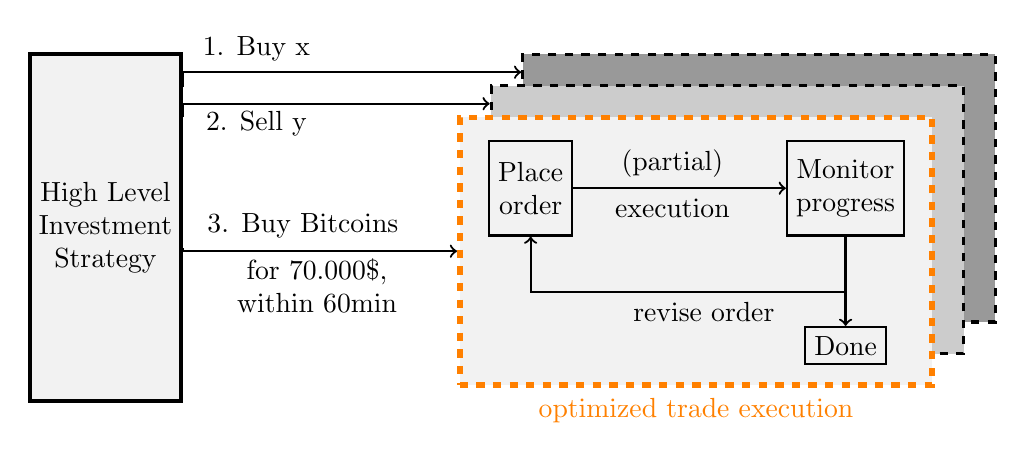
\begin{tikzpicture}[node distance = 16em, auto, thick]
    \node[draw, minimum height=4.4cm, align=center, fill=black!5, line width=0.5mm] at (0, -0.5)   (A) {High Level\\Investment\\Strategy};
    \node[draw, black, dashed, minimum height=3.4cm, minimum width=6cm, line width=0.4mm, fill=black!40] at (8.3,0) (X2) {};
    \draw[->] (A.61) node[above, xshift=2.7cm] {}  node[above, align=center, xshift=0.93cm, yshift=0.2cm]{1. Buy x}  |- (X2.154);
    
    \node[draw, black, dashed, minimum height=3.4cm, minimum width=6cm, line width=0.4mm, fill=black!20] at (7.9,-0.4) (X1) {};
    \draw[->] (A.55.9) node[above, xshift=2.7cm] {}  node[below, align=center, xshift=0.93cm, yshift=0.2cm]{2. Sell y} |- (X1.154);

    \node[draw, orange, dashed, minimum height=3.4cm, minimum width=6cm, line width=0.7mm, fill=black!5, label={below, orange: optimized trade execution}] at (7.5,-0.8) (X) {}; 

    \node[draw, minimum height=1.2cm, align=center] at (5.4, 0)   (B) {Place\\order};
    \node[draw, minimum height=1.2cm, align=center] at (9.4, 0)   (C) {Monitor\\progress};
    \node[draw, align=center] at (9.4, -2)   (D) {Done};
    
    \draw[->] (A.-15) node[above, xshift=1.52cm] {3. Buy Bitcoins}  node[below, align=center, xshift=1.7cm]{for $70.000\$$,\\within 60min} |- (X);
    \draw[->] (C.south) node[below, xshift=-1.8cm, yshift=-0.7cm] {revise order}  -- ++(-0,0) -- ++(0,-0.7) -| (B);
    \draw[->] (C.south)  -- (D);
    \draw[->] (B) node[above, xshift=1.8cm] {(partial)} node[below, xshift=1.8cm] {execution}  -- (C);

\end{tikzpicture}
}
\end{figure}
\end{overlayarea}
\end{frame}



\begin{frame}[fragile]{Optimized Trade Execution}
\begin{overlayarea}{\textwidth}{14\baselineskip}

%Maximal profit may be realized through multiple factors
%\begin{itemize}
%\item \emph{High level strategies} exploit profitable opportunities
%\item \emph{Optimized trade execution} minimize inevitably occurring costs.
%\end{itemize}\vspace{0.1cm}

Trading algorithm aims to \textbf{minimize inevitably occurring} costs:\\
\begin{itemize}
\item \emph{Fees} charged by the market place organizer
\item \emph{Hidden costs} in form of worsening prices
\end{itemize}\vspace{0.1cm}%\pause



In its simplest form the problem is defined by a particular financial instrument, which must be bought or sold within a fixed time horizon, while minimizing the expenditure for doing so.

\begin{figure}[ht]

	\centering
	\scalebox{0.7}{
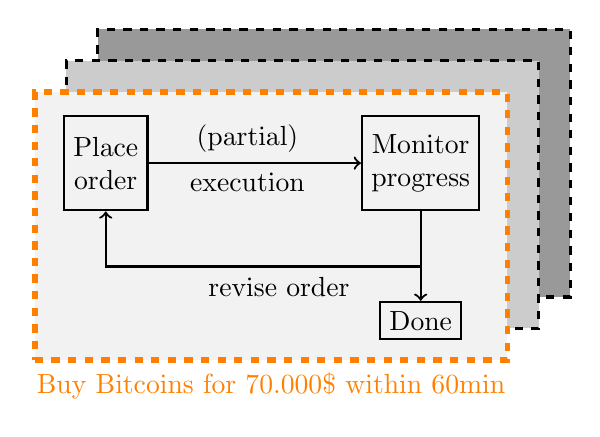
\begin{tikzpicture}[node distance = 16em, auto, thick]

    \node[draw, black, dashed, minimum height=3.4cm, minimum width=6cm, line width=0.4mm, fill=black!40] at (8.3,0) (X2) {};
    \node[draw, black, dashed, minimum height=3.4cm, minimum width=6cm, line width=0.4mm, fill=black!20] at (7.9,-0.4) (X1) {};
    \node[draw, orange, dashed, minimum height=3.4cm, minimum width=6cm, line width=0.7mm, fill=black!5, label={below, orange: Buy Bitcoins for $70.000\$$ within 60min}] at (7.5,-0.8) (X) {}; 

    \node[draw, minimum height=1.2cm, align=center] at (5.4, 0)   (B) {Place\\order};
    \node[draw, minimum height=1.2cm, align=center] at (9.4, 0)   (C) {Monitor\\progress};
    \node[draw, align=center] at (9.4, -2)   (D) {Done};
    
% 3. Buy Bitcoins for $70.000\$$,\\within 60min
    \draw[->] (C.south) node[below, xshift=-1.8cm, yshift=-0.7cm] {revise order}  -- ++(-0,0) -- ++(0,-0.7) -| (B);
    \draw[->] (C.south)  -- (D);
    \draw[->] (B) node[above, xshift=1.8cm] {(partial)} node[below, xshift=1.8cm] {execution}  -- (C);

\end{tikzpicture}
}
\end{figure}
\end{overlayarea}
\end{frame}


\begin{frame}[fragile]{Objectives \& Contributions}
\begin{overlayarea}{\textwidth}{14\baselineskip}

The following contributions to the problem of optimized trade execution have been made:
\begin{itemize}
\item A full-featured reinforcement learning environment for the simulation of trade execution is presented: The \emph{Orderbook Trading Simulator}.
\item An existing, \emph{backward learning} reinforcement learning approach has been examined and was improved in detail.
\item A novel, \emph{forward oriented} reinforcement learning approach is presented. It applies growing batch learning, samples from a continuous state space and outperforms the foremost algorithm.
\end{itemize}

\end{overlayarea}
\end{frame}

\begin{frame}{Outline of Contents}
  \setbeamertemplate{section in toc}[sections numbered]
  \tableofcontents[hideallsubsections]
\end{frame}



%%%%% TRADING BASICS %%%%%

\section{Trading Basics}

\begin{frame}[fragile]{Trading}
\begin{overlayarea}{\textwidth}{14\baselineskip}

Assets are typically traded through one of two basic market types:\vspace{0.5cm}\pause

Over-The-Counter (OTC) Markets
\begin{itemize}
\item Transactions take place directly between two parties.
\item Prices are negotiated directly between buyers and sellers.
\end{itemize}\vspace{0.2cm}\pause

Exchange Markets
\begin{itemize}
\item Transactions are executed by a \textbf{broker}.
\item Prices are determined by \textbf{Supply \& Demand}.
\begin{itemize}
\item Sellers can \textbf{ask} a price, they are aiming to make.
\item Buyers can \textbf{bid} a price, they are willing to pay.
\item \emph{Asks} and \emph{Bids} are maintained in a Limit Order Book.
\end{itemize}


\end{itemize}\vspace{0.2cm}

% Modern markets are fully electronically organized.

\end{overlayarea}
\end{frame}

\begin{frame}[fragile]{Limit Order Book}
\begin{overlayarea}{\textwidth}{14\baselineskip}
%Most exchange markets are based on the auction market model.

%\begin{itemize}
%\item Buyers can \textbf{bid} a price they are willing to pay.
%\item Sellers can \textbf{ask} a price they are aiming to make.
%\item The difference between \emph{best bid price} and \emph{best ask price} is called \textbf{bid-ask spread}
%\end{itemize}\pause\vspace{2mm}

The \textbf{Limit Order Book} (LOB) reflects supply ({\color{red}asks}) and demand ({\color{mygreen}bids}).\vspace{-5mm}
\begin{table}
\begin{subfigure}{.5\textwidth}
\scalebox{0.535}{
\begin{tabular}{|rrcrrr|}
\toprule
{} &  \text{Amount} &    Type &  \text{Volume} &  \text{VolumeAcc} &  \text{norm\_Price} \\
\midrule
\color{red}31.00 &   \color{red}200.0 &     \color{red}ask &  6200.0 &     8425.0 &    1.074533 \\
\color{red}30.00 &    \color{red}50.0 &     \color{red}ask &  1500.0 &     2225.0 &    1.039871 \\
\color{red}\textbf{29.00} &    \color{red}\textbf{25.0} &     \color{red}\textbf{ask} &   725.0 &      725.0 &    1.005208 \\
28.85 &     NaN &  center &     NaN &        NaN &         NaN \\
 \color{mygreen}\textbf{28.70} &    \color{mygreen}\textbf{200.0} &     \color{mygreen}\textbf{bid} &  5740.0 &     5740.0 &    0.994810 \\
 \color{mygreen}28.50 &    \color{mygreen}100.0 &     \color{mygreen}bid &  2850.0 &     8590.0 &    0.987877 \\
 \color{mygreen}28.00 &    \color{mygreen}300.0 &     \color{mygreen}bid &  8400.0 &    16990.0 &    0.970546 \\
\bottomrule
\end{tabular}}
\end{subfigure}%
\begin{subfigure}{.6\textwidth}
   \includegraphics[width=\textwidth]{images/intro_orderbook1.pdf}
\end{subfigure}
\end{table}


\vspace{0mm}\pause

\textbf{bid-ask spread}: Difference between \emph{best bid price} and \emph{best ask price}

\end{overlayarea}
\end{frame}


\begin{frame}[fragile]{Limit Order Book: 60 Minute interval}

\begin{figure}[ht]
	\centering
	\begin{subfigure}[t]{0.5\textwidth}
        		\centering
        		\includegraphics[width=\textwidth]{content/drawings/orderbook_window17}
        		\caption{Average market price.}
		\label{fig:orderbookwindow:avg}
    	\end{subfigure}%
	\begin{subfigure}[t]{0.5\textwidth}
        		\centering
        		\includegraphics[width=\textwidth]{content/drawings/orderbook_window17_worst}
        		\caption{Worst market price.}
		\label{fig:orderbookwindow:worst}
    	\end{subfigure}%

\end{figure}

Prices and Orderbooks permanently change:\\

\begin{itemize}
\item Order fulfillments (Trade execution)
\item Order cancelations
\item Order arrivals
\item Order updates ($+/-$ volume)
\end{itemize}

\end{frame}


\begin{frame}[fragile]{Trading costs}
\begin{overlayarea}{\textwidth}{14\baselineskip}

Investors must expect certain costs:
\begin{itemize}
\item \textbf{Fees} and \textbf{commissions} are contractually regulated.\\
$\Rightarrow$  Fix costs, predictable to a large extend.

\item \textbf{Slippage} is the deviation from the expected price.\\


E.g. large orders can have a major impact on Supply \& Demand.
\begin{itemize}
\item Diminishing availability, worsening prices, \ldots{}
\end{itemize}
\end{itemize}




\begin{table}
\scalebox{0.6}{
\begin{tabular}{|rrcrrr|}
\toprule
{} &  \text{Amount} &    Type &  \text{Volume} &  \text{VolumeAcc} &  \text{norm\_Price} \\
\midrule
\color{red}31.00 &   \color{red}200.0 &     \color{red}ask &  6200.0 &     8425.0 &    1.074533 \\
\color{red}30.00 &    \color{red}50.0 &     \color{red}ask &  1500.0 &     2225.0 &    1.039871 \\
\color{red}29.00 &    \color{red}25.0 &     \color{red}ask &   725.0 &      725.0 &    1.005208 \\
28.85 &     NaN &  center &     NaN &        NaN &         NaN \\
 \color{mygreen}28.70 &    \color{mygreen}200.0 &     \color{mygreen}bid &  5740.0 &     5740.0 &    0.994810 \\
 \color{mygreen}28.50 &    \color{mygreen}100.0 &     \color{mygreen}bid &  2850.0 &     8590.0 &    0.987877 \\
 \color{mygreen}28.00 &    \color{mygreen}300.0 &     \color{mygreen}bid &  8400.0 &    16990.0 &    0.970546 \\
\bottomrule
\end{tabular}}
\end{table}
\end{overlayarea}
\end{frame}


\begin{frame}[fragile]{Hidden Costs: Slippage}

Placing small orders, chances are high to get a good price. Larger orders \emph{eat} into the book and are fulfilled at successively worse price levels.

\begin{table}
\centering
\scalebox{0.6}{
\begin{tabular}{|rrcrrr|}
\toprule
{} &  \text{Amount} &    Type &  \text{Volume} &  \text{VolumeAcc} &  \text{norm\_Price} \\
\midrule
\color{red}31.00 &   \color{red}200.0 &     \color{red}ask &  6200.0 &     8425.0 &    1.074533 \\
\color{red}30.00 &    \color{red}50.0 &     \color{red}ask &  1500.0 &     2225.0 &    1.039871 \\
\color{red}29.00 &    \color{red}25.0 &     \color{red}ask &   725.0 &      725.0 &    1.005208 \\
28.85 &     NaN &  center &     NaN &        NaN &         NaN \\
 \color{mygreen}28.70 &    \color{mygreen}200.0 &     \color{mygreen}bid &  5740.0 &     5740.0 &    0.994810 \\
 \color{mygreen}28.50 &    \color{mygreen}100.0 &     \color{mygreen}bid &  2850.0 &     8590.0 &    0.987877 \\
 \color{mygreen}28.00 &    \color{mygreen}300.0 &     \color{mygreen}bid &  8400.0 &    16990.0 &    0.970546 \\
\bottomrule
\end{tabular}}


\scalebox{0.7}{
\begin{tabular}{l|l|r}
\textbf{20 shares:} & 150 shares: & 500 shares\\
\hline
Buy 20 @ 29 & Buy 25 @ 29\$ & Buy 25 @ 29\$\\
& Buy 50 @ 30\$ & Buy 50 @ 30\$\\
& Buy 75 @ 31\$ & Buy 200 @ 31\$\\
& & Buy 100 @ 31.50\$ \\
& & Buy 75 @ 32\$\\
& & Buy 50 @ 33\$\\
\hline
580\$ & 4,549.50\$ & 15,625\$\\
\hline
Avg: 29\$ & Avg: 30.33\$ & Avg: 31.25\$\\
Slippage: 0.00\$ & Slippage 1.33 \$ & Slippage 2.25 \$ \\
Cost: 0.00\$ & Cost 200 \$ & Cost 1,125 \$
\end{tabular}}
\end{table}
\end{frame}











\begin{frame}[fragile]{Order types: Simple Market Order}
\begin{overlayarea}{\textwidth}{14\baselineskip}

Scenario: You want to buy 100 shares of AIWC.

\begin{table}
\centering
\scalebox{0.6}{
\begin{tabular}{|lrlrrr|}
\toprule
{} &  Amount &    Type &  Volume &  VolumeAcc &  norm\_Price \\
\midrule

\color{mymauve}31.00 &   \color{mymauve}200.0 &     ask &  6200.0 &     8425.0 &    1.074533 \\
\color{mygreen}30.00 &    \color{mygreen}50.0 &     ask &  1500.0 &     2225.0 &    1.039871 \\
\color{red}29.00 &    \color{red}25.0 &     ask &   725.0 &      725.0 &    1.005208 \\
28.85 &     NaN &  center &     NaN &        NaN &         NaN \\
28.70 &   200.0 &     bid &  5740.0 &     5740.0 &    0.994810 \\
28.50 &   100.0 &     bid &  2850.0 &     8590.0 &    0.987877 \\
28.00 &   300.0 &     bid &  8400.0 &    16990.0 &    0.970546 \\
\bottomrule
\end{tabular}}
\end{table}

Solution: Buy them right away for the current market price:
\begin{itemize}
\item from {\color{red}Alice}:   $\Rightarrow 25*29\$ = 725\$$
\item from {\color{mygreen}Bob and Cedar}:   $\Rightarrow (20+30)*30\$ = 1500\$$
\item from {\color{mymauve}David}:   $\Rightarrow 25*31\$ = 775\$$
\end{itemize}
Total: 3000\$ (avg price: 30\$)
\vspace{2mm}

\emph{Fast, but costly (Average price differs from best price)}

$\Rightarrow$ Slippage of 1\$/share $\Rightarrow$ Loss of 100\$ compared to best ask.

\end{overlayarea}
\end{frame}


\begin{frame}[fragile]{Order types: Limit Order}
\begin{overlayarea}{\textwidth}{14\baselineskip}

Scenario: You want to buy 100 shares of AIWC, at max 30\$/share.

\only<1>{
\begin{table}
\centering
\scalebox{0.6}{
\begin{tabular}{|lrlrrr|}
\toprule
{} &  Amount &    Type &  Volume &  VolumeAcc &  norm\_Price \\
\midrule
31.00 &   200.0 &     ask &  6200.0 &     8425.0 &    1.074533 \\
\color{red}30.00 &    \color{red}50.0 &     \color{red}ask &  \color{red}1500.0 &     \color{red}2225.0 &    \color{red}1.039871 \\
\color{red}29.00 &    \color{red}25.0 &     \color{red}ask &   \color{red}725.0 &      \color{red}725.0 &    \color{red}1.005208 \\
28.85 &     NaN &  center &     NaN &        NaN &         NaN \\
28.70 &   200.0 &     bid &  5740.0 &     5740.0 &    0.994810 \\
28.50 &   100.0 &     bid &  2850.0 &     8590.0 &    0.987877 \\
28.00 &   300.0 &     bid &  8400.0 &    16990.0 &    0.970546 \\
\bottomrule
\end{tabular}}
\end{table}

Solution: Place a limit order (i.e. a \emph{bid}): BUY 100 @30\$

{\color{red}75} shares are matched immediately.}


\only<2>{
\begin{table}
\centering
\scalebox{0.6}{
\begin{tabular}{|lrlrrr|}
\toprule
{} &  Amount &    Type &  Volume &  VolumeAcc &  norm\_Price \\
\midrule
32.00 &    75.0 &     ask &  2400.0 &    11750.0 &    1.049274 \\
31.50 &   100.0 &     ask &  3150.0 &     9350.0 &    1.032879 \\
31.00 &   200.0 &     ask &  6200.0 &     6200.0 &    1.016485 \\
30.50 &     NaN &  center &     NaN &        NaN &         NaN \\
\color{mygreen}30.00 &    \color{mygreen}25.0 &     \color{mygreen}bid &   \color{mygreen}750.0 &      \color{mygreen}750.0 &    \color{mygreen}0.983695 \\
28.70 &   200.0 &     bid &  5740.0 &     6490.0 &    0.941068 \\
28.50 &   100.0 &     bid &  2850.0 &     9340.0 &    0.934510 \\
\bottomrule
\end{tabular}}
\end{table}

Solution: Place a limit order (i.e. a \emph{bid}): BUY 100 @30\$

75 shares are matched immediately.

{\color{mygreen}25}  remaining orders are added to orderbook and wait for matching offers.

\begin{itemize}
\item from Alice:   $\Rightarrow 25*29\$ = 725\$$
\item from Bob and Cedar:   $\Rightarrow (20+30)*30\$ = 1500\$$
\end{itemize}
Total: 2225\$ (avg price: 29.67\$)

\vspace{2mm}

\emph{Reduced Slippage, but not guaranteed to execute fully}
}

\end{overlayarea}
\end{frame}


\begin{frame}[fragile]{Order strategy: Submit and Revise}
\begin{overlayarea}{\textwidth}{14\baselineskip}

Combination of Market Order and Limit Order:
\begin{itemize}
\item Place limit order at t=[0, 15, 30, 45] and leave it for 15 minutes
\item At t=59 replace Limit Order with Market Order
\item Accepting more slippage towards end of period
\begin{itemize}
\item Check trade progresse very 15 minutes
\end{itemize}
\end{itemize}

\begin{itemize}
\item Exploit Market/Orderbook Features
\begin{itemize}
\item spread size
\item bid/ask imbalance (more people trying to sell or to buy?)
\item current market price 
\end{itemize}
\end{itemize}\pause

Idea: Use Reinforcement Learning to find optimal limits



\end{overlayarea}
\end{frame}







%%%%% ORDERBOOK TRADING SIMULATOR %%%%%

\section{Orderbook Trading Simulator}


\begin{frame}[fragile]{Historic Order Book Data}
\begin{overlayarea}{\textwidth}{14\baselineskip}

Most research is based on large data sets
\begin{itemize}
\item complete logs: order arrivals, cancelations, updates, matches
\item years of 'stock exchange' data (resolution: milliseconds)
\end{itemize}\pause

I work on
\begin{itemize}
\item Self recorded data from \textbf{Poloniex} (Digital Assets Market Place):
\item Orderbook \emph{snapshots} between Nov 10th 2016 and May 31st 2017\\
{\footnotesize 9 Currencypairs: \lstinline[basicstyle=\scriptsize]{'USDT_BTC', 'BTC_ETH', 'BTC_XMR', 'BTC_XRP', 'BTC_FCT', 'BTC_NAV', 'BTC_DASH', 'BTC_MAID', 'BTC_ZEC'}}
\item Datasize: \textasciitilde30KB per snapshot (resolution: 1 minute)
\end{itemize}

  {\footnotesize{Call \url{https://poloniex.com/public?command=returnOrderBook&currencyPair=USDT_BTC&depth=5000}}}

  \begin{lstlisting}[frame=single, breaklines=true, basicstyle=\footnotesize, belowskip=-1.0 \baselineskip]
{"asks":[["705.450000",2.772181],["706.170000",0.052838], ... ], "bids":[["705.000000",0.158232],["703.700000",0.001250], ... ], "isFrozen": 0, "seq": 63413296}  \end{lstlisting}
\end{overlayarea}
\end{frame}


\begin{frame}[fragile]{Historic Order Book Data (2): Bitcoins}
\begin{overlayarea}{\textwidth}{14\baselineskip}
\begin{figure}[ht]
	\centering
   \includegraphics[width=1.\textwidth]{content/drawings/bitcoin_historicPrices}\\
	Historic BTC prices between Nov, 10th 2016 and May, 31 2017.
\end{figure}
\end{overlayarea}
\end{frame}




%\begin{frame}[fragile]{Preprocessing}
%\begin{overlayarea}{\textwidth}{14\baselineskip}
%
%To restrict wasteful memory usage:
% \begin{itemize}
%  \item Almost identical price levels are round and merged:
%  \[ 2.772181 * 705.45\$ =
%  \begin{cases}
%    0.139212 * 705.450000\$\\
%    2.632969 * 705.450196\$\\
%  \end{cases}
%\]
%  \item ask and bid books are capped just above 100 bitcoins:\\
%  i.e. $70.000\$$ market order volume or 100-140 price levels per book.
%  \item Erroneous orderbook snapshots are discarded
%  \end{itemize}\vspace{5mm}\pause
%  
%  Datasize reduction: 30KB $\Rightarrow$ 6.6KB.\\
%  December 2016: 44.640 USDT/BTC snapshots (1.35GB $\Rightarrow$ 295MB).
%
%
%\end{overlayarea}
%\end{frame}




\begin{frame}[fragile]{Orderbook Trading Simulator (OTS)}
\begin{overlayarea}{\textwidth}{14\baselineskip}
Task: Buy 100 bitcoins over a period of 4*15=60 minutes
\begin{lstlisting}[basicstyle=\scriptsize]
ots = OrderbookTradingSimulator(orderbooks=window_60orderbooks, volume=100, tradingperiods=4, periodlength=15)

summary = ots.trade(limit=713.0)  # t=0
summary = ots.trade(limit=715.0)  # t=15
display(ots.history)  # Slippage: 340.85$
\end{lstlisting}\vspace{-1cm}\pause

\begin{itemize}
\item maintains a \emph{masterbook}.\vspace{2mm}
\includegraphics[width=0.7\textwidth]{content/images/masterbook_adjustments}\pause
\item returns detailed trading statistics
\end{itemize}\vspace{-0.8cm}


\begin{table}
\centering
\scalebox{0.42}{
\begin{tabular}{|lrrrrrrrrrrrlrrrr|}
\toprule
{} &     ASK &     BID &  CENTER &  SPREAD &  LIMIT &  VOLUME &  vol\_traded &      CASH &  cash\_traded & ... &     avg & forced &  initMAvg &     low &    high &  cost \\
\midrule
03:01 &  711.42 &  709.74 &  710.58 &    1.68 &  713.0 &  100.00 &          46.77 &      0.00 &    -33280.72 & ... &  711.51 &  False &            718.42 &  711.42 &  713.00 &     43.48 \\
03:16 &  712.52 &  711.86 &  712.19 &    0.66 &  715.0 &   53.23 &          28.90 & -33280.72 &    -20630.99 & ... &  713.99 &  False &            718.42 &  712.52 &  715.00 &     98.53 \\
03:31 &  715.10 &  712.98 &  714.04 &    2.12 &  717.5 &   24.33 &           6.68 & -53911.71 &     -4780.95 & ... &  716.16 &  False &            718.42 &  715.10 &  717.41 &     37.28 \\
03:46 &  718.60 &  717.77 &  718.18 &    0.83 &  720.0 &   17.65 &          17.65 & -58692.66 &    -12706.15 & ... &  719.73 &  False &            718.42 &  718.60 &  720.00 &    161.57 \\
\bottomrule
\end{tabular}}
\end{table}

\end{overlayarea}
\end{frame}


\begin{frame}[fragile]{Orderbook Trading Simulator (OTS): Implementation}
\begin{overlayarea}{\textwidth}{14\baselineskip}
\begin{figure}[ht]
	\centering
   \includegraphics[width=0.8\textwidth]{content/drawings/trading_example17_good}
	\caption{Visualization of an exemplary trading strategy.}
	\label{fig:tradingstrategy17good}
\end{figure}

\end{overlayarea}
\end{frame}

%\begin{frame}[fragile]{Orderbook Trading Simulator (OTS): Drawbacks}
%\begin{overlayarea}{\textwidth}{14\baselineskip}
%
%\begin{itemize}
%\item Can not distinguish between a limit order being removed and a limit order being updated to a new price level.
%\item Competitors reactions on large orders are not accounted for.
%\item Orderbooks on a minutely basis miss a great part of the markets volatility.
%\item Hidden Orders are not accounted for.
%\end{itemize}
%
%\end{overlayarea}
%\end{frame}









%%%%% REINFORCEMENT LEARNING APPROACHES %%%%%

\section{Reinforcement Learning Approaches}





\begin{frame}[fragile]{Reinforcement Learning Framework}
\begin{overlayarea}{\textwidth}{14\baselineskip}

Use RL to find optimal limits for Submit \& Revise Strategies.
\begin{description}
\item[Actions] current\_best + $[-0.4, -0.3, ... , 0.9, 1.0]$ \%\\
{\small ask=$705.45$, $a=+0.1 \Rightarrow$ $limit=705.45 * 1.001 = 706.16$}\pause
\item[Costs] Difference between expected and obtained price (Slippage)\\
cost = {\color{red}vol\_traded} * ({\color{mygreen}avg\_paid} - {\color{blue}initial\_center})\\
$cost = {\color{red}17.65} * ({\color{mygreen}719.73} - {\color{blue}710.58}) = \textbf{161.57}$
\end{description}\vspace{-6mm}

\begin{table}
\centering
\scalebox{0.42}{
\begin{tabular}{|lrrrrrrrrrrrlrrrr|}
\toprule
{} &     ASK &     BID &  CENTER &  SPREAD &  LIMIT &  VOLUME &  vol\_traded &      CASH &  cash\_traded & ... &     avg & forced &  initMAvg &     low &    high &  cost \\
\midrule
03:01 &  711.42 &  709.74 &  \color{blue}710.58 &    1.68 &  713.0 &  100.00 &          46.77 &      0.00 &    -33280.72 & ... &  711.51 &  False &            718.42 &  711.42 &  713.00 &     43.48 \\
03:16 &  712.52 &  711.86 &  712.19 &    0.66 &  715.0 &   53.23 &          28.90 & -33280.72 &    -20630.99 & ... &  713.99 &  False &            718.42 &  712.52 &  715.00 &     98.53 \\
03:31 &  715.10 &  712.98 &  714.04 &    2.12 &  717.5 &   24.33 &           6.68 & -53911.71 &     -4780.95 & ... &  716.16 &  False &            718.42 &  715.10 &  717.41 &     37.28 \\
03:46 &  718.60 &  717.77 &  718.18 &    0.83 &  720.0 &   17.65 &          \color{red}17.65 & -58692.66 &    -12706.15 & ... &  \color{mygreen}719.73 &  False &            718.42 &  718.60 &  720.00 &    \textbf{161.57} \\
\bottomrule
\end{tabular}}
\end{table}\pause

\begin{description}
\item[States] \emph{remaining time}, \emph{remaining volume}, [orderbook features, ...]\pause
\item[Goal] Minimize expected costs
\end{description}

\end{overlayarea}
\end{frame}


\begin{frame}[fragile]{Backward Approach}
\begin{overlayarea}{\textwidth}{14\baselineskip}

\begin{itemize}
\item Proposed by Nevmyvaka et al. in 2006 \cite{Nevmyvaka:2006}.
\item Q-learning and dynamic programming
\item Samples discretized state space in a backward, brute force manner.
\end{itemize}\vspace{-4mm}

\only<1-4>{
\begin{figure}
\begin{subfigure}{.7\textwidth}
\centering
\scalebox{0.6}{\hspace{-4cm}
\begin{algorithm}[H] 


     \SetAlgoLined
     \footnotesize
     
     \KwIn{V=70.000\$, H=60min, T=4, I=[12.5\%..100\%], L=[-4..10]}

\For{t=1 to T}{
    \While{not end of data}{
        Transform (orderbook) $\rightarrow o_1..o_R$\;
        \For{i=0 to I}{
            \For{a=0 to L}{
                 Set $x = [t, i, o_1, ..., o_R]$\;
                    Simulate transition $x \rightarrow y$\;
                    Calculate immediate $\text{cost}_{im}(x, a)$\;
                    Look up argmax $\text{cost}(y, p)$\;
                    Update $\text{cost}([t, v, o_1, ..., o_R], a)$\;

            }
        }
        Select the highest-payout action argmax $\text{cost}(y, p)$ in every state $y$ to output optimal policy
    }
}
\end{algorithm}}
\end{subfigure}%
\begin{subfigure}{.5\textwidth}\pause
\hspace{-2cm}
\includegraphics[width=1\textwidth]{content/drawings/heatmap_3months_t1}\pause\\

\vspace{-0.5cm}
\hspace{-2cm}
\includegraphics[width=1\textwidth]{content/drawings/heatmap_3months_t2}\pause\\

\vspace{-0.5cm}
\hspace{-2cm}
\includegraphics[width=1\textwidth]{content/drawings/heatmap_3months_t3}
\end{subfigure}%
\end{figure}}

\only<5>{
\begin{figure}
\centering
\includegraphics[width=1\textwidth]{content/drawings/heatmap_3months}\\
Trained over: 4.154 periods � 60 minutes (Nov 2016 - Apr 2017)\\

states = [time\_left, volume\_left]\\
32 states, 15 actions = 480 trials per period
\end{figure}
}

\end{overlayarea}
\end{frame}



\begin{frame}[fragile]{Backward Approach - Discussion (1)}
\begin{overlayarea}{\textwidth}{14\baselineskip}

Subject of Trade
\begin{itemize}
\item Nevmyvaka: Buy 100 shares
\item Here: Buy shares for $70.000\$$
\end{itemize}

\begin{figure}[ht]
	\centering
   \includegraphics[width=0.6\textwidth]{content/drawings/bitcoin_historicPrices}
\end{figure}
\end{overlayarea}
\end{frame}

\begin{frame}[fragile]{Backward Approach - Discussion (2)}
\begin{overlayarea}{\textwidth}{14\baselineskip}

Action limit mapping
\begin{itemize}
\item Nevmyvaka: Forced crossing of the bid-ask spread.
\item Here: no crossing, action=0 guarantees partial execution.
\end{itemize}

\lstinline!limit_buy = ask * (1 + (a/1000))! instead of \lstinline!limit_buy = bid + a!\\

\lstinline!limit_sell = bid * (1 - (a/1000))! instead of \lstinline!limit_sell = ask - a!,\\
{\small where $a \in [-4, -3, ... , +9, +10]$}

\begin{table}
\centering
\scalebox{0.6}{
\begin{tabular}{|lrlrrr|}
\toprule
{} &  Amount &    Type &  Volume &  VolumeAcc &  norm\_Price \\
\midrule

31.00 &   200.0 &     ask &  6200.0 &     8425.0 &    1.074533 \\
30.00 &    50.0 &     ask &  1500.0 &     2225.0 &    1.039871 \\
\color{red}29.00 &    25.0 &     \color{red}ask &   725.0 &      725.0 &    1.005208 \\
28.85 &     NaN &  center &     NaN &        NaN &         NaN \\
\color{mygreen}28.70 &   200.0 &     \color{mygreen}bid &  5740.0 &     5740.0 &    0.994810 \\
28.50 &   100.0 &     bid &  2850.0 &     8590.0 &    0.987877 \\
28.00 &   300.0 &     bid &  8400.0 &    16990.0 &    0.970546 \\
\bottomrule
\end{tabular}}
\end{table}



\end{overlayarea}
\end{frame}


\begin{frame}[fragile]{Backward Approach - Discussion (3)}
\begin{overlayarea}{\textwidth}{14\baselineskip}

Discrete State Space
\begin{itemize}
\item No generalization to states never observed.
\item Rounding required in learning process.
\begin{itemize}
\item Loss of accuracy
\item Cost scaling problem:\\
Non-linear slippage growth.
\end{itemize}
\end{itemize}

\begin{figure}[ht]
	\centering
   \includegraphics[width=0.3\textwidth,trim={0 0.2cm 0 0.7cm},clip]{content/drawings/nonlinearcosts}
\end{figure}
\end{overlayarea}
\end{frame}

\begin{frame}[fragile]{Backward Approach - Discussion (4)}
\begin{overlayarea}{\textwidth}{14\baselineskip}

Markov Property
\begin{itemize}
\item States capture all relevant information from history.
\end{itemize}

Nevmyvaka: Backward approach does not incorporate preceding trades.\vspace{5mm}

E.g., if starting at t=45 and a remaining trade volume of $17.500\$$:

\begin{figure}[ht]
	\centering
	\begin{subfigure}[t]{0.3\textwidth}
        		\centering
        		\includegraphics[width=\textwidth]{content/drawings/masterbook_customstart_NoSim}
        		\caption{Original Orderbook.}
		\label{fig:differingmasterbooks:NoSim}
    	\end{subfigure}
	\begin{subfigure}[t]{0.3\textwidth}
        		\centering
        		\includegraphics[width=\textwidth]{content/drawings/masterbook_customstart_SimMarketOrder}
        		\caption{Assuming 52.500 shares being matched at \lstinline!t=0!, then no further matches.}
		\label{fig:differingmasterbooks:SimMarketOrder}
    	\end{subfigure}%
	\begin{subfigure}[t]{0.3\textwidth}
        		\centering
        		\includegraphics[width=\textwidth]{content/drawings/masterbook_customstart_SimEqual}
        		 \caption{Assuming 52.500 shares being matched evenly at 1.166 shares per minute.}
		\label{fig:differingmasterbooks:SimEq}
    	\end{subfigure}%
\end{figure}

\end{overlayarea}
\end{frame}




%%%%% DISCUSSION AND EXPERIMENTS %%%%%

\section{Experiments}

\begin{frame}[fragile]{Data \& Task}
\begin{overlayarea}{\textwidth}{14\baselineskip}

Data
\begin{itemize}
\item Currency pair: USDT/BTC
\item Training period: Nov 10th, 2016 - Apr, 30th 2017: 4154 orderbook windows � 60min.
\item Test period: May 2017: 724 orderbook windows
\end{itemize}

Task:
\begin{itemize}
\item Buy Bitcoins worth of $70.000\$$
\item Trading horizon: 60min
\item 4 order revisions (i.e. period length=15min)
\item 8 inventory levels ($8.750\$, ..., 70.000\$$)\\
Sample transitions, collected in backward mode:\\
$\Rightarrow 4.154 * 4 * 8 * 15 = \textbf{1.993.920}$ \textbf{samples}
\end{itemize}

\end{overlayarea}
\end{frame}

\begin{frame}[fragile]{Baseline}
\begin{overlayarea}{\textwidth}{14\baselineskip}
\begin{itemize}
\item Simple Market Order
\item Optimal Submit \& Leave strategie: a=4\only<2>{ and a=2}
\end{itemize}


\only<1>{
\begin{figure}[ht]
        	\centering
        	\includegraphics[width=0.8\textwidth]{content/drawings/bestActionTrain}\\
	\small Average Submit \& Leave costs over the full training period.
	\label{fig:bestAction}
\end{figure}}
\only<2>{
\begin{figure}[ht]
	\centering
	\begin{subfigure}[b]{0.5\textwidth}
        		\centering
        		\includegraphics[width=\textwidth]{content/drawings/runningMean240_MarketPrice}
        		\caption{Observed Market Order Slippage.}
		\label{fig:runningmean:marketPrice}
    	\end{subfigure}%
	\begin{subfigure}[b]{0.5\textwidth}
        		\centering
        		\includegraphics[width=\textwidth]{content/drawings/runningMean240_bestAction}
        		\caption{Best S\&L action.}
		\label{fig:runningmean:bestaction}
    	\end{subfigure}

\end{figure}
}


\end{overlayarea}
\end{frame}

\begin{frame}[fragile]{Backward Approach: Additional Market Variables}
\begin{overlayarea}{\textwidth}{14\baselineskip}
\begin{figure}[ht]
	\centering
	\includegraphics[width=\textwidth]{content/drawings/bw_additionalMarketVariables}
\end{figure}
Only \emph{spread} is beneficial.
\end{overlayarea}
\end{frame}

\begin{frame}[fragile]{Backward Approach: Look-ahead Variables}
\begin{overlayarea}{\textwidth}{14\baselineskip}
\begin{figure}[ht]
	\centering
	\includegraphics[width=\textwidth]{content/drawings/bw_lookahead}
\end{figure}
Massive performance gain.
\end{overlayarea}
\end{frame}

%\begin{frame}[fragile]{Backward Approach: Constant Market Variables}
%\begin{overlayarea}{\textwidth}{14\baselineskip}
%\begin{figure}[ht]
%	\centering
%	\includegraphics[width=\textwidth]{content/drawings/bw_constantVars}
%\end{figure}
%\end{overlayarea}
%\end{frame}

\begin{frame}[fragile]{Backward Approach: Simulation of Proceeding trades}
\begin{overlayarea}{\textwidth}{14\baselineskip}
\begin{figure}[ht]
	\centering
	\includegraphics[width=\textwidth]{content/drawings/bw_simPre}
\end{figure}
$-2.76\% \Rightarrow -4.55\%$ [Volume, Time]\\
$-8.93\% \Rightarrow -9.70\%$ [Volume, Time, Spread]


\end{overlayarea}
\end{frame}

\begin{frame}[fragile]{Backward Approach: Action Consequences}
\begin{overlayarea}{\textwidth}{14\baselineskip}
\begin{figure}[ht]
	\centering
	\includegraphics[width=\textwidth]{content/drawings/bw_actionConseq}
\end{figure}
No improvement


\end{overlayarea}
\end{frame}



\begin{frame}[fragile]{Backward Approach: Function Approximation}
\begin{itemize}
\item RandomForestRegressor: BatchTree-agent
\item 150 Trees
\end{itemize}

\begin{overlayarea}{\textwidth}{14\baselineskip}
\begin{figure}[ht]
	\centering
	\includegraphics[width=\textwidth]{content/drawings/bw_approx}
\end{figure}
VolTimeSpread: {\color{red}terrible} performance\\
Single a*-feature: loss in performance\\
All a*-features simultaneously: {\color{mygreen}improvement} of $-7.53\%$


\end{overlayarea}
\end{frame}


\begin{frame}[fragile]{Forward Approach}
\begin{overlayarea}{\textwidth}{14\baselineskip}

Idea: Collect more realistic transitions
\begin{itemize}
\item Simulate \textbf{full} trades
\item Include trade history
\item Sample from continuous state space
%\item Extract orderbook features on the go
\end{itemize}\pause\vspace{-4mm}

%Exploration phase:
%\begin{itemize}
%\item Apply $\epsilon$-greedy strategy repeatedly
%\item Enforce non-repeating paths
%\end{itemize}
%
%Retrain agent after 256 exploration phases

\begin{figure}
\centering
\scalebox{0.7}{
\begin{algorithm}[H] 

     \SetAlgoLined
     \footnotesize
     
     \KwIn{data, V=$70.000\$$, H=60min, T=4, L=[-4..10], E=60, retrain=256}

Shuffle(data)\;
Split data into chunks of length $retrain$

\While{not end of chunks}{
\For{orderbook window in chunks}{
Init OTS(orderbook\_window, V, H, T, L)\\
    \For{epoch=0 to E}{
        Reset OTS to $V=100\%$ and random time point (in H)\\
        \Repeat{$V=0\%$}{
        Set $x_t=[\text{time\_left}, \text{volume\_left}, o_1, ..., o_R]$\\
        Enquire $\epsilon$-greedy action from model\\
        \If{action chain led to an end state previously}{choose other action}
        Apply action\\
        Remember transition \{$x_t, action, cost, x_{t+1}$\}
        }
    }
    Retrain model from collected transitions (growing batch)
    }
}

\label{alg:forward:pseudocode}
\end{algorithm}}
\end{figure}

\end{overlayarea}
\end{frame}


\begin{frame}[fragile]{Forward Approach Performance}
\begin{overlayarea}{\textwidth}{14\baselineskip}

\begin{figure}[ht]
	\centering
	\includegraphics[width=\textwidth]{content/drawings/BT_Forward_Performance}
\end{figure}

\end{overlayarea}
\end{frame}



%%%%% CONCLUSION %%%%%

\section{Conclusion}
\begin{frame}[fragile]{Conclusion}
\begin{overlayarea}{\textwidth}{14\baselineskip}

\begin{figure}[ht]

	\centering
	\scalebox{0.7}{
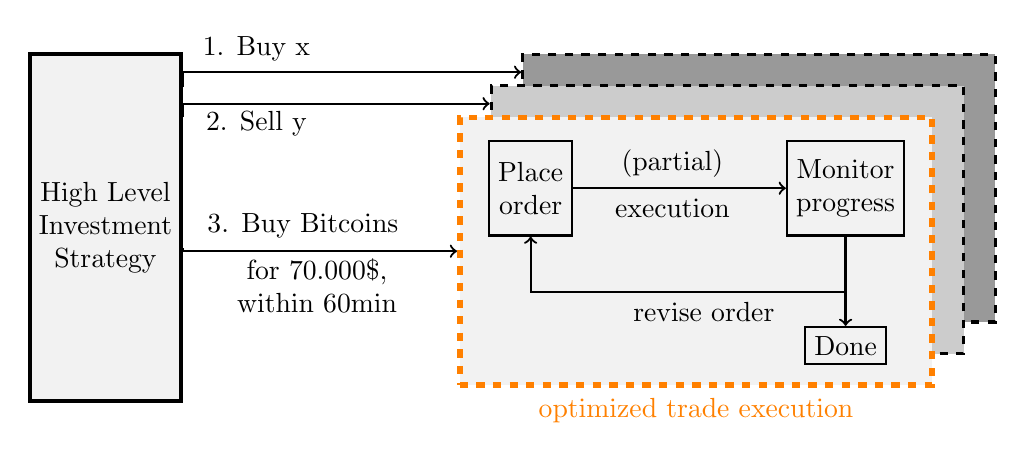
\begin{tikzpicture}[node distance = 16em, auto, thick]
    \node[draw, minimum height=4.4cm, align=center, fill=black!5, line width=0.5mm] at (0, -0.5)   (A) {High Level\\Investment\\Strategy};
    \node[draw, black, dashed, minimum height=3.4cm, minimum width=6cm, line width=0.4mm, fill=black!40] at (8.3,0) (X2) {};
    \draw[->] (A.61) node[above, xshift=2.7cm] {}  node[above, align=center, xshift=0.93cm, yshift=0.2cm]{1. Buy x}  |- (X2.154);
    
    \node[draw, black, dashed, minimum height=3.4cm, minimum width=6cm, line width=0.4mm, fill=black!20] at (7.9,-0.4) (X1) {};
    \draw[->] (A.55.9) node[above, xshift=2.7cm] {}  node[below, align=center, xshift=0.93cm, yshift=0.2cm]{2. Sell y} |- (X1.154);

    \node[draw, orange, dashed, minimum height=3.4cm, minimum width=6cm, line width=0.7mm, fill=black!5, label={below, orange: optimized trade execution}] at (7.5,-0.8) (X) {}; 

    \node[draw, minimum height=1.2cm, align=center] at (5.4, 0)   (B) {Place\\order};
    \node[draw, minimum height=1.2cm, align=center] at (9.4, 0)   (C) {Monitor\\progress};
    \node[draw, align=center] at (9.4, -2)   (D) {Done};
    
    \draw[->] (A.-15) node[above, xshift=1.52cm] {3. Buy Bitcoins}  node[below, align=center, xshift=1.7cm]{for $70.000\$$,\\within 60min} |- (X);
    \draw[->] (C.south) node[below, xshift=-1.8cm, yshift=-0.7cm] {revise order}  -- ++(-0,0) -- ++(0,-0.7) -| (B);
    \draw[->] (C.south)  -- (D);
    \draw[->] (B) node[above, xshift=1.8cm] {(partial)} node[below, xshift=1.8cm] {execution}  -- (C);

\end{tikzpicture}
}
\end{figure}\pause

Goal: Minimize hidden costs (MarketOrder in may 2017: $\approx277.49\$$)
\begin{itemize}
\item Submit \& Leave Strategy: $0.00\%$ ($-44.18\%$)\pause
\item Backward approach by Nevmyvaka et al.: $-4.84\%$   ($-46.88\%$)\pause
\item Backward approach improved: $-9.70\%$    ($-49.59\%$)\pause
\item Forward approach: $-11.41\%$    ($-50.55\%$)
\end{itemize}

\end{overlayarea}
\end{frame}

\begin{frame}[fragile]{Future Work}
\begin{overlayarea}{\textwidth}{14\baselineskip}

Orderbook Trading Simulator
\begin{itemize}
\item Different data: high resolution log files
\end{itemize}\vspace{1cm}\pause

Forward Learning Approach
\begin{itemize}
\item (Deep) neural networks and replay memory
\item Continuous action space
\item Combine with specialized time series prediction methods\\
e.g. Prevedex STaR \cite{STAR}
\end{itemize}

\end{overlayarea}
\end{frame}


\begin{frame}[standout]
  Questions?
\end{frame}

\appendix


\begin{frame}[fragile]{Volatiliy of USDT/BTC and (USDT/Pound}
\begin{overlayarea}{\textwidth}{14\baselineskip}

\begin{figure}[ht]
	\centering
	\includegraphics[width=0.9\textwidth]{content/images/BitcoinVolatility}\\
	\scriptsize Source: \url{https://99bitcoins.com/bitcoin-volatility-explained}
	\label{fig:bitcoinvolatility}
\end{figure}
\end{overlayarea}
\end{frame}



\begin{frame}[fragile]{Performance of forward agent}
\begin{overlayarea}{\textwidth}{14\baselineskip}
\begin{figure}[ht]
	\centering
	\includegraphics[width=\textwidth]{content/drawings/fw_performance}
\end{figure}
\end{overlayarea}
\end{frame}

\begin{frame}[fragile]{The circuit of masterbook adjustments}
\begin{overlayarea}{\textwidth}{14\baselineskip}
\begin{table}
\scalebox{0.7}{\centering
\begin{tabular}{l|l|l|l|l|l}
\toprule
{} &     t=0 &     t=1 &  t=2 &  t=3 &  t=4\\
\midrule
ob[t] & \pbox{20cm}{705.45: 3.17 \\ 707.18: 7.99} & \pbox{20cm}{705.45: 5.04 \\ 707.18: 1.53} & \pbox{20cm}{705.45: 6.85 \\ 707.18: 1.53} &    \pbox{20cm}{705.45: 5.08 \\ 707.18: 7.77}  &  \pbox{20cm}{705.45: 6.84 \\ 707.18: 7.77} \\[3ex]
\hline
diff = \\ob[t]-ob[t-1] & \pbox{20cm}{705.45: +3.17 \\ 707.18: +7.99} & \pbox{20cm}{705.45: +1.87 \\ 707.18: -6.45} & \pbox{20cm}{705.45: +1.81} &    \pbox{20cm}{705.45: -1.77 \\ 707.18: +6.24}  & \pbox{20cm}{705.45: +1.75}   \\[3ex]
\hline
master = \\ master + diff & \pbox{20cm}{705.45: 3.17 \\ 707.18: 7.99} & \pbox{20cm}{705.45: 1.87 \\ 707.18: 1.53} & \pbox{20cm}{705.45: 1.81 \\ 707.18: 1.53}  &   \pbox{20cm}{{\color{gray}705.45: -1.77} \\ 707.18: 7.77\\ drop negatives}  & \pbox{20cm}{705.45: 1.75 \\ 707.18: 7.77}  \\[3ex]
\hline
\\trade now & \pbox{20cm}{705.45: 3.17} & \pbox{20cm}{705.45: 1.87} & \pbox{20cm}{705.45: 1.81} &   - & \pbox{20cm}{705.45: 1.75} \\[3ex]
\hline
\\traded total & \pbox{20cm}{705.45: 3.17} & \pbox{20cm}{705.45: 5.04} & \pbox{20cm}{705.45: 6.85} &   - & \pbox{20cm}{705.45: 8.6} \\[3ex]
\hline
master = \\ master - trade & \pbox{20cm}{707.18: 7.99} & \pbox{20cm}{707.18: 1.53} & \pbox{20cm}{707.18: 1.53} &    \pbox{20cm}{707.18: 7.77}  & \pbox{20cm}{707.18: 7.77} \\[3ex]

\bottomrule
\end{tabular}

}
\caption{The circuit of masterbook adjustments}
\label{tab:otssim}
\end{table}


\end{overlayarea}
\end{frame}






\begin{frame}[allowframebreaks]{References}


  \bibliography{demo}
  \bibliographystyle{abbrv}

\end{frame}

\end{document}
